% * <feiyu19901122@gmail.com> 2015-11-06T18:59:49.627Z:
%
% ^.
\documentclass[10pt,twocolumn,letterpaper]{article}

\usepackage{cvpr}
\usepackage{times}
\usepackage{epsfig}
\usepackage{graphicx}
\usepackage{amsmath}
\usepackage{amssymb}
\usepackage{multirow}
\usepackage{color}
\usepackage{array}
\newcolumntype{L}[1]{>{\raggedright\let\newline\\\arraybackslash\hspace{0pt}}m{#1}}
\newcolumntype{C}[1]{>{\centering\let\newline\\\arraybackslash\hspace{0pt}}m{#1}}
\newcolumntype{R}[1]{>{\raggedleft\let\newline\\\arraybackslash\hspace{0pt}}m{#1}}
\usepackage{mathtools}


\makeatletter
\renewcommand\paragraph{\@startsection{paragraph}{4}{\z@}%
           {1.25ex \@plus1ex \@minus.2ex}%
           {-1em}%
           {\normalfont\normalsize\bfseries}}
            
\renewcommand\subsubsection{\@startsection{subsubsection}{3}{\z@}%
                {-2ex\@plus -1ex \@minus -.2ex}%
                {0.1ex \@plus .2ex}%
                {\normalfont\normalsize\bfseries}}
                
                
% Include other packages here, before hyperref.

% If you comment hyperref and then uncomment it, you should delete
% egpaper.aux before re-running latex.  (Or just hit 'q' on the first latex
% run, let it finish, and you should be clear).
\usepackage[pagebackref=true,breaklinks=true,letterpaper=true,colorlinks,bookmarks=false]{hyperref}

%\cvprfinalcopy % *** Uncomment this line for the final submission

\def\cvprPaperID{1798} % *** Enter the CVPR Paper ID here
\def\httilde{\mbox{\tt\raisebox{-.5ex}{\symbol{126}}}}

% Pages are numbered in submission mode, and unnumbered in camera-ready
\ifcvprfinal\pagestyle{empty}\fi
\begin{document}

%%%%%%%%% TITLE
%\title{Creating Album Highlights Automatically}
\title{Event-specific Image Importance}



\author{First Author\\
Institution1\\
Institution1 address\\
{\tt\small firstauthor@i1.org}
% For a paper whose authors are all at the same institution,
% omit the following lines up until the closing ``}''.
% Additional authors and addresses can be added with ``\and'',
% just like the second author.
% To save space, use either the email address or home page, not both
\and
Second Author\\
Institution2\\
First line of institution2 address\\
{\tt\small secondauthor@i2.org}
}

\maketitle
%\thispagestyle{empty}

%%%%%%%%% ABSTRACT
\begin{abstract}
When creating a photo album of an event, people typically select a few important images to keep or share. There is some consistency in the process of choosing the important images, and discarding the unimportant ones. Modeling this selection process will assist automatic photo selection and album summarization. In this paper, we show that the selection of important images is consistent among different viewers, and that this selection process is related to the event type of the album. We introduce the concept of event-specific image importance. We collected a new event album dataset with human annotation of the relative image importance with each event album. We also propose a Convolutional Neural Network (CNN) based method to predict the image importance score of a given event album, using a novel rank loss function and a progressive training scheme. Results demonstrate that our method significantly outperforms various baseline methods.

 
\end{abstract}

%%%%%%%%% BODY TEXT
\section{Introduction}
With the proliferation of cameras (in cell phones and other portable cameras), taking photographs is practically effortless, and happens frequently in everyday life. When attending an event, for instance, a Thanksgiving holiday, participants often take many photos recording every interesting moment during the event. This leads to an oversized album at the end of the event. When we need to simplify the album before saving to a device, or if we want to make a photo collage or a photo book to share our important moment %(for example, our wedding ceremony) 
with others, we have to go through the tedious and time-consuming work of selecting important images from a large album. Therefore, it is desirable to perform this task automatically.

% Moreover, it's often the case that we take photos that are not interesting to keep anymore when we look back at the album, such as photos of food. 

%When we save the album to device, the tedious and time-consuming work of manually cleaning up the album often makes us leave the large album disordered and redundant as it is, and this often leads to our reluctancy to look back at this oversized album in the future.

%On the other hand, if we want to make a photo collage or a photo book to share our important moment (for example, our wedding ceremony) with others, we have to go through the tedious work of selecting important images from the large album. This is even true with photos taken by professional photographers, because most of the time the album is much larger and redundant than what we want to keep.

%Both the need of keeping and sharing photo albums lead to the need to select an important subset of images from a larger album automatically, and it's desirable to keep the user input as little as possible.

Automatic photo selection or album summarization has been studied by some researchers \cite{nips_summarize, vacation, sum_pinaki, photo_selection1, gaze}. They aim at personal event albums, and visual content information as well as diversity and coverage is often considered jointly to obtain a summarization. 
However, these works ignored the role of the event type in the selection process. Intuitively, the event type of the album is an important criterion when we select important images. For example, if we need to select important photos from a vacation to Hawaii, the photo of the volcano on the Big Island is definitely important to keep, whereas if the album is a wedding ceremony, beautiful scenes are only background and are not likely to be more important than the shot of the bride and groom. 

In this paper, we introduce the concept of event-specific image importance. It is different from general image interestingness or aesthetics, in that it is contextual, and is based on the album the image is in. We focus on the event-specific importance score of a single image, and do not consider summarization problems where diversity and coverage are also important: Image importance prediction is the most challenging and crucial part of the event curation/album summarization process; Moreover, the importance score can be directly applied to to any album summarization algorithm. 
%Walber \etal showed with a user study that single image properties such as attractiveness and image interestingness are important criteria for humans to do photo selection, while diversity and coverage of the selection are less important \cite{gaze}. 
We collect an event-specific image importance dataset from human annotators, and we show that the event-specific importance is subjective yet predictable. Finally, we provide a method for predicting event-specific image importance using Convolutional Neural Network (CNN). We propose a new loss function and training procedure, and our CNN method greatly outperforms different baselines.

\section{Related Work}

\paragraph{Image properties.}
Importance of an image is a complex image property, and is related to many other image properties. Many image properties can be viewed as cues when selecting important images, such as memorability \cite{Isola2011, NIPS2011_4451}, specificity \cite{specificity}, popularity \cite{www14_khosla}, aesthetics and interestingness \cite{interesting, interesting2}. Those image properties are correlated to image contents, such as high level features: object and scene categories \cite{Isola2011, NIPS2011_4451, specificity, www14_khosla, interesting}, and low level features: texture, edge distribution, etc.\cite{interesting2, www14_khosla}. In this work, rather than the general image properties mentioned above, we study event-specific image importance, which summarizes human preferences related to images within the context of an album, where the album is of a known event type.

\paragraph{Convolutional Neural Networks(CNNs).}
The development of methods for training deep CNNs has led to rapid progress in many computer vision tasks in recent years.  Substantial improvements have been made in basic computer vision problems such as image classification \cite{imagenet, googlenet}, object detection \cite{rcnn, devil} and scene recognition \cite{places, scene}. Now, there is a greater focus on learning higher-level image properties. One example closely related to our project is Xiong \etal's work on event recognition from static images \cite{event_recognition}. In this work, the network is divided into different channels, creating human and object maps that are then fused with the original images to jointly train a deep architecture that predicts the event type from a single image. Our model also uses deep representations to capture event features, but our  focus is on event curation rather than event recognition. In fact, our model assumes that the event type is known. Event curation then requires choosing the most important images for the event in question.

%Without the context of an album, general high level properties of one image are studied by several works. \cite{Isola2011, NIPS2011_4451} show that memorability is correlated to object and scene category, and enclosed space and human presence increase memorability of an image. Image popularity also correlates with object categories \cite{www14_khosla}. \cite{specificity} shows image specificity is correlated to image content, and correlated to memorability as well. \cite{interesting} uses high level attributes to predict aesthetics.  \cite{interesting2} shows interestingness is predictable from several cues. Rather than general image properties, we study human preference to images with a context of an album and with the information of event type of the album. 

\paragraph{Album summarization and photo selection.}
The most closely related work to our project is on summarization and selection from an album or several albums.

Event summarization of public photo/video collections involves selecting the most important moments of a social event from a variety sources on the web\cite{social_summarize, scene_summarize}. Here, the goal is to retrieve all of the important moments (diversity), while covering the whole event (coverage). More relevant to this project is work that attempts to summarize a single album \cite{nips_summarize,vacation, sum_pinaki}. Again, coverage and diversity of the albums are considered, and single image importance is used as a cue\cite{vacation, sum_pinaki}. Sinha \etal aim at summarization of personal photo collections taken over a long time span, take the event type as one photo descriptor to calculate diversity and coverage of the photo subset \cite{sum_pinaki}. %Instead, we focus on an album taken from a single event, and we use event type information when predicting image importance.

For the photo selection problem, 
Yeh \etal proposed a ranking system for photographs based on a set of aesthetic rules and personal preferences \cite{perosnalized_che}. 
%YUFEI: WHAT IS THEIR TECHNIQUE? DO THEY USE MACHINE LEARNING?
%This work is for photography, not personal albums.  
Walber \etal use gaze information from user's photo viewing process to assist the automatic photo selection algorithm, so this work requires eyetracking\cite{gaze}. The work by Ceroni \etal \cite{photo_selection1} is probably most relevant to our work. It focuses on selection of important photos from a single event album, and different factors are considered: image quality, presence of faces, concept features, and collection based features such as album size. However, each album used for training and testing in this work is collected from a single participant, and the important subset is picked by the same person: it does not focus on common human preferences. 
%Also, it does not take event type as a factor, and the albums in the dataset are mostly vacation albums. 
Moreover, the prediction algorithm is tested on unseen images in the same album used for training, and it does not focus on new album prediction.



%The work that is most related to our project is work on summarization and selection from an album or several albums\cite{social_summarize, scene_summarize}. For example, using public photo/video collections from the internet for well-known cities such as Rome, the objective is to automatically derive a one page visual summary of a scene or city that captures the key sites of interest\cite{scene_summarize}. This is accomplished by clustering the images based on visual features, such as SIFT.
%{\LARGE Stopped here on the review of previous work - I need to move on to the methods and results!}\cite{nips_summarize} focuses on single album summarization, and they consider coverage and diversity of the albums and do not take image importance score as a cue. \cite{vacation, sum_pinaki} study the problem of summarization of personal albums, using  image quality as well as coverage and diversity as cues. Single image quality is only one of the factors, and image quality is general aesthetics or interestingness which does not take event-specific information into account. \cite{sum_pinaki} aims at summarization of personal photo collections taken in a long time span, and it takes event type as one photo descriptor to calculate diversity and coverage of the photo subset. Instead, we focus on an album taken from a single event, and we use event type information for image importance score prediction.
%\cite{perosnalized_che} proposed a ranking system for photographs based on a set of aesthetic rules and personal preference. Their work is for photography, not personal albums. \cite{gaze} uses gaze information from user's photo viewing process to assist automatic photo selection algorithm, and their work needs additional gaze information from user which is hard to acquire.

%\cite{photo_selection1} is most relevant to our work. In their work, they aim on selection for important photos from single event album, and different factors are considered: image quality, face presentation, concept features, and collection based features. However, each album used for training and test in this work is collected from single participant and the important subset is picked by the same person: it does not focus on the common human preference. Also, it does not take event type as a factor, and the albums in the dataset are most vacation albums. Moreover, the prediction algorithm is tested on unseen images in the same album used for training, and it does not focus on new album prediction. 

Our work differs from all the above in that we focus on: i) whether humans have common preferences for image importance/preference scores, ii) whether image importance can be predicted for unseen albums with widely varying content, and iii) whether event type information is important for the prediction. To summarize, we are introducing a subjective but predictable image property: event-specific image importance, and we propose a method to predict this property.
\section{The  Curation of Flickr Events Dataset}

\begin{table*}[t]
\begin{center}
\small
\centerline{
\begin{tabular}{|  C{2cm} | C{3cm} | C{4.5cm} | C{3.5cm} | C{2.8cm} | }
\hline
\textbf{Categories}                & \textbf{Important Personal Event} & \textbf{Personal Activity} & \textbf{Personal Trip} & \textbf{Holiday} \\ \hline\hline
\textbf{Event types} \newline \textbf{and \# albums} &  Wedding:198 (98\%) \newline Birthday:180 (91\%)\newline Graduation:178 (88\%)
&Protest:50 (92\%)  \newline Personal Music Activity:25 (92\%) \newline Religious Activity:50 (90\%)\newline  Casual Family Gather:50 (84\%) \newline Group Activity:50 (82\%) \newline Personal Sports:100 (78\%)\newline Business Activity:50 (76\%)\newline Personal Art Activity:54 (70\%)
           &  Architecture/Art:50 (92\%)\newline  Urban Trip:100 (89\%)\newline Cruise Trip:50 (88\%) \newline Nature Trip:50 (86\%)\newline Theme Park:100 (86\%)\newline Zoo:99 (85\%) \newline Museum:50 (84\%)\newline  Beach Trip:50 (82\%)  \newline Show:100 (82\%)\newline  Sports Game:50 (58\%) 
             &   Christmas:100 (87\%)\newline Halloween:99 (86\%) \\ \hline
\end{tabular}
}
\end{center}
\caption{23 Event types, their corresponding number of albums, and percentage of significant albums at level $q=0.05$ using Kendall's $W$ statistics. The event types fall into four categories.}
\vspace{-0.15in}
\label{event_type}
\end{table*}
Are people's ratings for images in albums representing particular events predictable? Our intuition is that in an album of a certain event type, there will be a consistent subset of images that will be preferred by most people. However, there is no available dataset to verify this intuition, or to test the degree of people's agreement on this highly subjective task. In this section, we describe the collection of the CUration of Flickr Events Dataset (CUFED), and measure the consistency of human subjects' preferences on this dataset. CUFED provides a ground truth dataset that allows us to measure the predictability of human rated image importance scores, and to develop our prediction model. CUFED will be made available to public. 
\subsection{Album Collection}
In order to collect a dataset of albums of different event types, we segmented albums from the Yahoo Flickr Creative Commons 100M Dataset (YFCC100M ) \cite{thomee2015yfcc100m}. The YFCC100M Dataset has 100 million images and videos from Flickr. In this collection, each image has the following metadata: the user ID who uploaded this photo; the time the image was taken; and often there are user tags. We took advantage of the metadata to segment dataset into albums: For each photo uploader, events are segmented based on timestamps and tags: images taken within short time interval (3 hours) and with more than 1/3 common tags belong to one event. Using tags to filter the data was inspired by the observation that users tend to give the same tags to an event album instead of individually tagging every single image in it. Using this approach, we segmented 1.8 million albums from the YFCC100M dataset. Here, we randomly selected 20,000 albums to work with. 

To get the event type of those albums, we presented the albums to workers on Amazon Merchanical Turk (AMT) and asked them to classify the albums into 23 event types. Aside from these event types, the workers could choose ``Other events", ``Not an event", ``More than a single event" or ``Cannot decide" instead of available event types. We chose our 23 event types so that they cover the most common events in our lives, ranging from weddings to sports games. %, and the event types
All 23 event types are shown in Table~\ref{event_type}. Each album was labeled by 3 workers. Over 82\% of the 20k albums received the same labels from at least 2 of the 3 workers. 
%We excluded the albums that at least one worker thought was ``Not an event". 
We kept the albums which were given the same label by 2 or more workers, and this label was given to the album. This resulted in 16,489 albums.
%assuming those albums to be not an event album. 

We further randomly selected 50-200 albums from each of the event types (except for \textit{Personal Music Activity}, which has 25 albums), resulting in a dataset of 1883 albums. The number of events of each type is shown in Table~\ref{event_type}. The size of the albums varies between 30 and 100 images. We chose these parameters by hand to emphasize our intuition that some event types will have more consistent ratings, and hence more predictability, than others.  Therefore, in this dataset, we emphasized those events in hope of learning more from them.
\subsection{Data Annotation}

In order to get the rating for each image in an album, we presented an album together with its event type to AMT workers and let them rate each image in that album as very important, important, neutral, or irrelevant. The four ratings are mapped to scores \{2,1,0,-2\} when creating ground truth. We intentionally did not give specific criteria for the rating levels, to encourage the workers to rate based on their intuition. In our pilot study, workers on AMT tended to mark a large proportion of the images as very important/important. This is understandable, since most of the albums are of high quality, but it leads to a ceiling effect on the ratings. To control the size of images marked as important, we forced the workers to label 5\%-30\% of the images as very important, and 10\%-50\% as important. The average time to rate each image was 7.7 seconds. Each album was annotated by 5 distinct workers. 292 workers participated in the tasks. Over 90\% of our data was annotated by 93 workers. 

The image ratings collected from AMT differed in quality among different AMT workers. To avoid low quality work,  only workers who passed an event recognition test using  single images could proceed to the real task. In addition, we added two distractor images per album which were clearly not related to the event in order to screen workers who were not paying attention. However, it  is not possible to assure the quality of an individual submission because of the subjective nature of the image importance rating task. Therefore, in order to filter ``bad" submissions, we found workers who consistently gave scores far from others and filtered out their submissions. If more than 30\% of his/her submissions had a euclidean distance from the average of other workers' submissions greater than a threshold, that worker's submissions were filtered out.  Only two workers were filtered out in this way.

%\begin{table*}[t]
%\begin{center}
%\small
%\begin{tabular}{|  C{2cm} | C{3cm} | C{4.5cm} | C{3.5cm} | C{2.8cm} | }
%\hline
%\textbf{Categories}                & \textbf{Important Personal Event} & \textbf{Personal Activity} & \textbf{Personal Trip} & \textbf{Holiday} \\ \hline\hline
%\textbf{Event types} \newline \textbf{and \# albums} &  Wedding:198 (98\%) \newline Birthday:180 (89\%)\newline Graduation:178 (87\%)

%&Protest:50 (94\%)  \newline Religious Activity:50 (92\%)\newline Personal Music Activity:25 (88\%) \newline Casual Family Gather:50 (86\%) \newline Group Activity:50 (82\%) \newline Personal Sports:100 (81\%)\newline Business Activity:50 (76\%)\newline Personal Art Activity:54 (70\%)
%           &   Cruise Trip:50 (88\%) \newline Nature Trip:50 (88\%)\newline Urban Trip:100 (87\%)\newline Zoo:99 (87\%)\newline Architecture/Art:50 (86\%)\newline Theme Park:100 (85\%)\newline Beach Trip:50 (84\%)\newline Museum:50 (80\%)\newline Show:100 (78\%)\newline  Sports Game:50 (62\%) 
%             &   Christmas:100 (86\%)\newline Halloween:99 (82\%) \\ \hline
%\end{tabular}
%\end{center}
%\caption{23 Event types, their corresponding number of albums, and percentage of significant albums at level $q=0.05$ using Kendall's $W$ statistics. The event types fall into four categories.}
%\label{event_type}
%\end{table*}


\subsection{Consistency Analysis}
\label{consistency_section}

To examine the consistency of the human ratings of images, we split our subjects into two independent groups of two and three raters for each album, and used Spearman's rank correlation ($\rho$) to evaluate their consistency. $\rho$ ranges from -1 (perfectly inverse correlation) to 1 (perfect correlation), while 0 indicates no correlation. For each album, we averaged the correlation scores of all possible random splits. The average correlation over all albums was 0.40. 

We further evaluated the annotation consistency with Kendall's $W$, which directly calculates the agreement among multiple raters, and accounts for tied ranks. Kendall's $W$ ranges from 0 (no agreement) to 1 (complete agreement). Note that in our workers' rating of one album, tied ranks are very frequent, since there are only 4 possible ratings, and the average album size is 52. Coincidentally, the average Kendall's $W$ over all albums was also 0.40. Both Spearman's rank correlation $\rho$ and Kendall's $W$ showed significant consistency across subjects despite the high subjectivity of this problem.

To test the statistical significance of Kendall's $W$ score, we did a permutation test over $W$ to obtain the distribution of $W$ under the null hypothesis, and for each event type, we used the Benjamini-Hochberg procedure to control the false discovery rate (FDR) for multiple comparisons \cite{Benjamini01thecontrol}. At level $q = 0.05$, 86\% of albums had significant agreement on average. Table~\ref{event_type} shows the percentage of albums with significant agreement for each event type. The different percentages of significant albums in different event types confirmed our intuition that some event types would be more consistently rated than others. The wedding event was the most consistently rated, with 98\% of albums being significantly consistent, while for the sports game category, only  58\% of the albums received significant consistency scores,  the lowest among the 23 events.  In the supplementary material, we include examples of albums that received high and low consistency ratings.
\section{Approach}
In this section, we propose a Convolutional Neural Network (CNN) based method for estimating an event-specific image importance score in an album, given the event type of this album. We use a siamese network \cite{siamese} with a novel rank loss function to take two images at a time and rank them relative to one another based on their scores.

\subsection{CNN Structure}
\label{CNN_section}
The design of our siamese CNN architecture is shown in Fig.~\ref{figure1}. It has several properties described in the following subsections.

\begin{figure*}[!htb]
\begin{center}
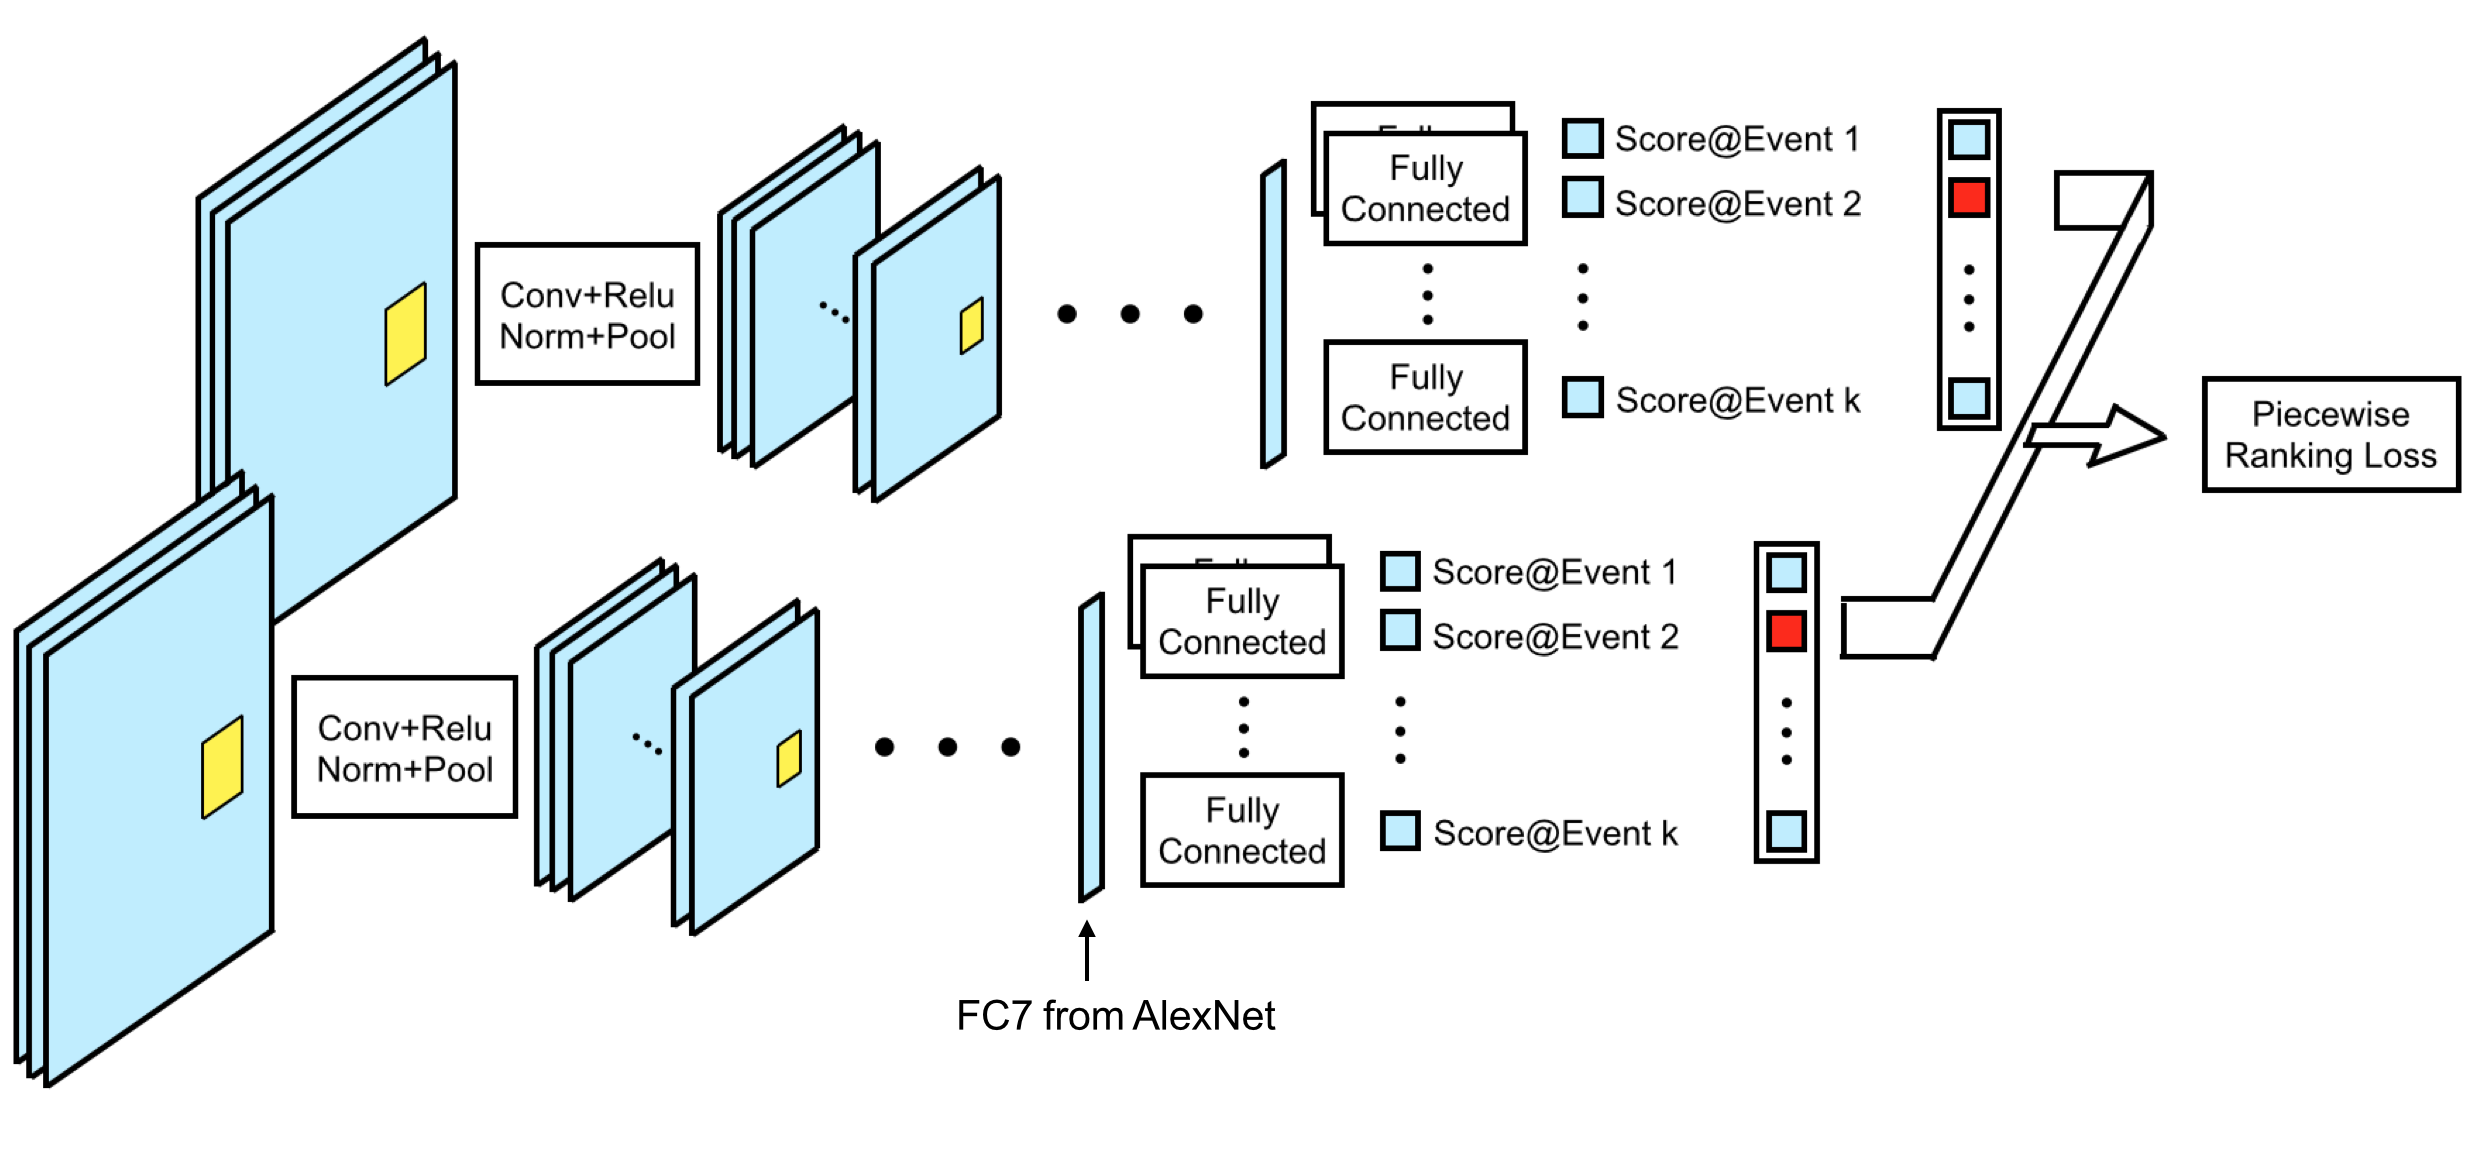
\includegraphics[width=6in]{architecture3}
\end{center}
\caption{A siamese CNN architecture for joint training over events. A pair of images from the same album is the input to the two pathways. Intermediate layers are omitted here for simplicity. The network computes an importance score for its input image; only the units corresponding to the correct event type are activated and back-propagated through (the red square represents a mask).}
\label{figure1}
\vspace{-0.15in}
\end{figure*}

\subsubsection{Feature sharing among event types}  
\label{section_1}
We train a single siamese network with albums from all event types. The last layer, however, has separate outputs for each event type. The reasons are as follows. First, there exists strong visual similarity among different event types in terms of image importance, therefore for a specific event type, labeled data from other event types will help as implicit data augmentation. Second, feature sharing will significantly reduce the number of parameters in the network and regularize the network training. Especially for our problem, high variance among albums within each event type and relatively small datasets make this even more necessary. Therefore, in our network, all event types share the features, while the output level has event-specific ratings. During the training process, only the output corresponding to the event type of an image pair receives an error signal, and we assume that we know the event type at test time.

\subsubsection{2-stage progressive training} 
Due to the large variation among albums and the relatively small scale of the dataset (especially for some event types such as \textit{casual family/friends gathering}), directly training a CNN for separate event types as in Section~\ref{section_1} may lead to over-fitting for some event types with less training data. Therefore, we use a 2-stage progressive learning method: we train all images with one output for the whole network; and then switch to training with a separate output for each event type.  Initialization of the second stage is done using the network from the first stage. This helps in that i) the features that are useful for all event types are learned first, using all of the data; ii)  the individual event-type output units are initialized with the weights from the one-output unit, so they already have some knowledge of what makes an important image; and iii) the discrimination is then refined based on the properties of individual event types. Some pictures are just excellent no matter what the occasion; our two-stage learning system leverages that intuition\footnote{We also tried to cluster the event types into $k$ ``superclasses" according to their similarity, and to use the superclass information for the first stage training. However, that didn't lead to a better result. One possible reason is that our event type clustering algorithm does not perform well.}. %By utilizing this, we set the initialization of 2-stage in a reasonable place. 

 \subsubsection{Siamese architecture} 

There is large variation in the quality of the albums within an event type, which might bias the judgment of participants in our AMT task. Therefore it is difficult to learn a reliable absolute image importance score that is suitable for different albums. Meanwhile, the relative importance ranking of images within the same album is more meaningful and more practical in applications. Hence, rather than training on an absolute image score, we use the average score difference between a pair of images from the same album to train the network. This is the motivation for using the siamese network architecture \cite{siamese}, which processes pairs of images. In the siamese network, the two pathways share weights, so a common representation is learned (see Fig.~\ref{figure1}).
 
\subsubsection{Piecewise ranking loss} 
For each input image pair to the network $(\text{I}_{1}, \text{I}_{2})$, $G(\text{I}_i)$ is the ground truth score of  image $\text{I}_i$, and $P(\text{I}_i)$ is its predicted score from the network. We use a piecewise ranking loss (PR loss) to train the network:

\begin{equation} 
  \text{PR} = \begin{cases}
 \frac{1}{2}\text{max}(0, \left | D_\text{p} \right |-\text{m}_\text{s})^{2} &\text{if}  \; D_\text{g} < \text{m}_\text{s}\\
\mathrlap{
\frac{1}{2}\left \{ \text{max}(0, \text{m}_\text{s}-D_\text{p})^{2}
+ \text{max}(0, D_\text{p}-\text{m}_\text{d})^{2} \right \}
} \\
 & \text{if} \;  \text{m}_\text{s} \leq D_\text{g}  \leq \text{m}_\text{d} \\
 \frac{1}{2}\text{max}(0, \text{m}_\text{d}-D_\text{p})^{2} \; \; \; \; \; \;  \; \;\; \;  \; \; \; \;   & \text{if}  \; D_\text{g}  > \text{m}_\text{d}
\end{cases}
\label{loss_function}
\end{equation}
\noindent
where  $D_\text{g} = G(\text{I}_{1})-G(\text{I}_{2})$ is the ground truth score difference between the input image pair, and  $D_\text{p} = P(\text{I}_{1})-P(\text{I}_{2})$ is the predicted score difference. $\text{m}_\text{s}$ and $\text{m}_\text{d}$ are predefined values for similar and different margins. In Equation ~\ref{loss_function}, several conditions are considered:

\begin{itemize}
  \item When $D_\text{g}  > \text{m}_\text{d}$, the loss function reduces to a variation of ranking SVM hinge loss \cite{ranking_loss}. We use L-2 loss which penalizes high errors more heavily than traditional hinge loss \cite{svm}. This is similar to contrastive loss function when the input pair of images are deemed dissimilar \cite{contrastive}, but we are not using the euclidean distance of the output of the network, since the sign of $D_\text{p}$ is important here. 
  \item When $D_\text{g} < \text{m}_\text{s}$, the loss function reduces to a variation of contrastive loss when the input pair is deemed similar \cite{contrastive}. In addition to the contrastive loss in \cite{contrastive}, we introduce a margin: $ \text{m}_\text{s}$. The margin serves as a slack term. The reason to have it is that the ground truth importance score is acquired from a group of humans, and the variance is relatively high among the humans, as shown in Section~\ref{consistency_section}. The introduction of relaxation with $\text{m}_\text{s}$ makes the network less sensitive to this variance in our ground truth.
  \item When $\text{m}_\text{s} < D_\text{g}  < \text{m}_\text{d}$, the loss function will only penalize the $D_\text{p}$ not being in the same range with $D_\text{g}$. This pulls $D_\text{p}$ towards $D_\text{g}$ when the image pair is similar in rating, reducing the loss function's vulnerability to the variance in our ground truth.
\end{itemize}

The PR objective loss function has the following advantages: Rather than training only on images with different ratings, it provides an error signal even when image pairs have the same rating, moving them closer together in representational space.  This makes full use of the training dataset. Our piecewise version also  introduces relaxation in the ground truth score, thus making the network more stable, which is beneficial when the ratings are subjective.

\subsection{Incorporating Face Heatmaps}
Images with faces tend to be more interesting than images without them\cite{sum_pinaki}. Moreover, our intuition is that in an event album, important people will appear more frequently. This across-album feature cannot be captured by a CNN trained with image pairs. In order to incorporate face information, we generate face heatmaps, and use them to train a shallow CNN to independently predict the importance score of the photos. A separate face heatmap-based score enables flexible tuning of the relative strength of the two scores from original images and face heatmaps. 

To generate the face heatmaps, we use a state-of-the-art face detection network \cite{Li_2015_CVPR}. In order modulate the heatmaps according to face frequency, we need facial identity information. We train 18 CNN models for different face parts and concatenate the final fully-connected layers as the final face descriptor, following a similar pipeline as \cite{Sun_2014_CVPR}. We then do agglomerative identity clustering to obtain the frequency of faces in an album. In the face heatmap, faces are represented  with Gaussian kernels, and the two most frequent faces are emphasized by doubling their peak values. These are used as input to a shallow siamese CNN trained from scratch, with one convolutional layer and two fully connected hidden layers, in the same manner as the image network. Details of the training and architecture are described in the supplementary material. 

% Moreover, peak value of Gaussian kernels is modulated by the quality score of that face. This is inspired by the observation that low quality faces are not as appealing as high quality faces.
Examples of face heatmaps are shown in Fig.~\ref{figure4}. In the testing stage, the prediction from the original image and the face heatmap network are combined according to the following formula:
\begin{equation}
P=P_{\text{I}} + {\lambda} \cdot \text{min}\left \{ \text{max}\left \{ P_{\text{f} }, \beta \right \},\alpha \right \}
\label{equa-face}
\end{equation}
where $(\text{P}_{\text{I}}, \text{P}_{\text{f}})$ are predicted scores from the original photo network and face heatmap network respectively. The face heatmap contains a limited information, therefore we constrain the effect of the face heatmap for the final prediction with $(\alpha, \beta)$, so that extreme predictions from the face heatmap are eliminated; $\lambda$ is also used to further control the effect of the face heatmap-based prediction. These parameters are set using cross-validation and a grid search.

\begin{figure}[h]
\begin{center}
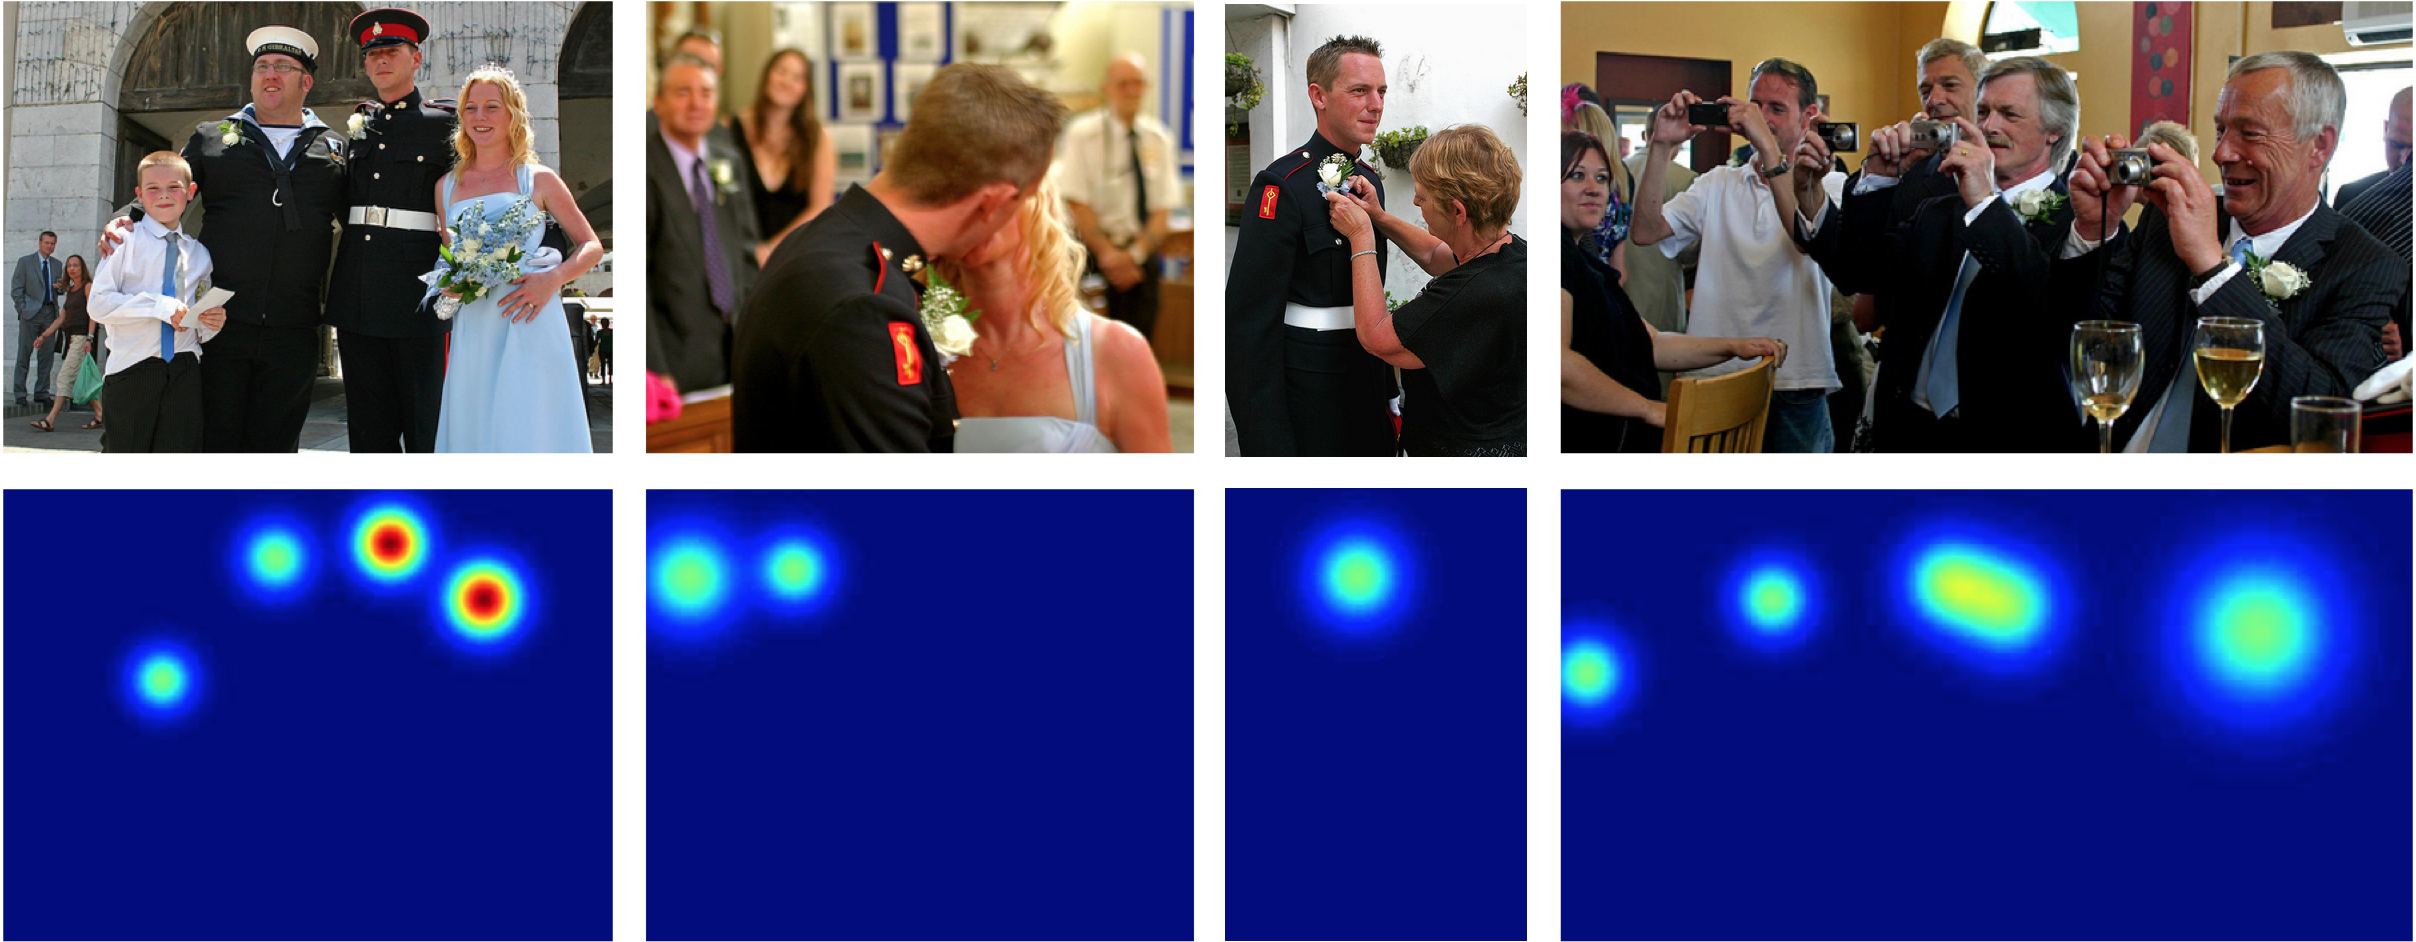
\includegraphics[width=3.1in]{section3_1}
\end{center}
\caption{Face heatmaps from a wedding event album. First row: original images; Second row: face heatmaps. Faces of the two most important people have higher peak values (red dots). The second column shows that face detection is not ideal; the  third column shows that identity clustering is not perfect, as the groom is not emphasized.}
\vspace{-0.2in}
\label{figure4}
\end{figure}

\section{Experimental Results}
In this section, we compare our results with several baseline methods.
\subsection{Experimental Settings}
\paragraph{Dataset}
For training and testing, we randomly split the  Curation of Flickr Events Dataset into 3:1 albums for every event type. The training set consists of 1404 albums, and the test set has 479 albums. 

\paragraph{Parameter setting}
We use Alexnet to initialize the CNN architecture and then fine-tune it \cite{imagenet,caffe}. In Fig.~\ref{figure1}, FC7 is from Alexnet, driving the event-specific sigmoidal score prediction layer. We assume we know the event type, and the teaching signal is masked by the correct event. For PR loss, we set $\text{m}_\text{s} = 0.1$ and $\text{m}_\text{d} = 0.3$. For training parameters, we use the default settings for pre-training in Caffe \cite{caffe}, but we start from a smaller learning rate of 0.001 \cite{rcnn}. 

We follow \cite{imagenet}'s data augmentation approach: Input images are resized to $256\times 256$. During the training stage, images are randomly cropped to $227 \times 227$ crops, and there is a 50\% probability that input images are horizontally flipped. In the test stage, predictions are averaged on five crops (four corners and the center) and their horizontal reflections. We train five different CNNs with 5-fold cross validation, and use an ensemble of the five networks for the final prediction. 
%The cross-validation ensemble can improve the generalization of the network by increasing the ambiguity \cite{ensemble}. %Increasing ambiguity??? In the first stage of our progressive learning, we use only one event cluster, which means all event types are categorized into one superclass. 



\paragraph{Evaluation metrics} 
We use two evaluation methods to compare the different approaches. For both evaluation methods, we assume that given an event album, we view the top $t\%$ images as relevant images, and measure the metric at various values of $t$.

First, we use mean average precision (MAP) to evaluate our models. MAP is a common evaluation method for information retrieval \cite{MAP}. It is the averaged area under the precision-recall curve over all albums. Given the collection of albums, and top $t\%$ of the images as being relevant images, $\text{MAP}@(t\%)$ can be calculated:
\begin{equation}
\textup{AP(S)}@t\%=\int_{0}^{1}p(r)d(r)\approx \frac{\sum_{k=1}^{n}p(k)\times \textup{rel}(k)}{\left \lceil n\cdot t\% \right \rceil}
\end{equation}
\begin{equation}
\textup{MAP(U)}@t\% = \frac{1}{N}\sum_{i=1}^{N}\textup{AP}(\textup{S}_{i})@t\%
\end{equation}
where $\text{S}_{i}$ is the $i$th album, and $\text{U}$ is the collection of all albums. $n$ is the size of album $S$,  $p(k)$ is the precision at rank $k$, and $\text{rel}$ is an indicator of whether the $k$th ranked image from our algorithm is a relevant image, i.e. among the top $t$
\% ground truth.

Second, we calculate the precision ($P$), the ratio between the number of relevant photos in the retrieved images over the total number of relevant images at each level of $t$. Unlike MAP, $P$ cares entirely about how many important images can be retrieved at a cut-off level, and does not care about the position they are in the retrieval list, or where the rest of important images are in the ranking system. Although less informative than MAP, $P$ is also an intuitive way to demonstrate the effectiveness of our predicted image ranking result. Since we are solving an image selection problem, we care more about MAP and $P$ for small $t\%$, so we only present results for $t \leq 30$.

\subsection{Results and Analysis}
In this section, we compare our method, Piecewise Ranking-CNN trained progressively (PR-CNN(Progressive)), on all event types to various baselines, and demonstrate the advantages of our method. 
Figure~\ref{figure5} is an example to show how our algorithm performs intuitively. Our result clearly learns meaningful concepts for the wedding event. More examples are shown in the supplementary material. The quantitative comparison of the methods, broken out into each of the 23 event types, is also shown in the supplementary material.  In the following sections, we describe the various baseline methods we benchmark our system against. To make a long story short, we achieve our best result using an ensemble of the five PR-CNN(Progressive) networks (See Table \ref{aesthetic_table}).
  

\begin{figure}[h]
\begin{center}
\includegraphics[width=3.1in]{result_image}
\end{center}
\caption{Example results for one wedding album. Top 5 images of the album from different methods are shown here. First row: Ground truth acquired from AMT workers; Second row: Our prediction using Ensemble-CNN; Third row: Random selection.}
\label{figure5}
\end{figure}

\subsubsection{Does aesthetics play an important role?}
In a user study, Walber \etal show that that humans use the visual appeal of an image as a criterion for selecting important images in an album \cite{gaze}. Here, in order to quantify the role attractiveness plays in the selection, we use an aesthetic score prediction method instead of the importance score. We  train a CNN classifier similar to \cite{aesthe_14}, using aesthetic scores collected using AMT.  

Table~\ref{aesthetic_table} shows that the aesthetic score of images is only slightly better than random. We conclude that aesthetics, at least using this method, is not a very important criterion for human selection of important images in event albums. In the supplementary material, we observe that the aesthetic score is more predictive for some events than others, e.g. \textit{Nature trip}, \textit{Personal art activity} (in which many photos are portrait shots). This is consistent with our intuition: aesthetics is an important criterion for human selection in events without strong narrative structure.

\begin{table*}[]
\begin{center}
\small
\centerline{
\begin{tabular}{c|cccccc|cccccc}
\hline
          & \multicolumn{6}{c|}{$\text{MAP}@t\%$}          & \multicolumn{6}{c}{$P@t\%$} \\ \hline  \hline
t\%       & 5     & 10    & 15    & 20    & 25    & 30    & 5  & 10  & 15 & 20 & 25 & 30 \\ \hline
Random & 0.122 & 0.164 & 0.211 & 0.260 & 0.305 & 0.350 & 0.058  &  0.093   &  0.141  &  0.195  & 0.251   & 0.298   \\
Worker & 0.328 & 0.410 & 0.476 & 0.531 & 0.580 & 0.624 & 0.242   &  0.371   &  0.448  &  0.505  & 0.552   & 0.591   \\ \hline
Aesthetic & 0.139 & 0.191 & 0.242 & 0.290 & 0.338 & 0.384 & 0.060   &  0.121   &   0.176 &    0.228&0.284    &    0.335\\ 
Pre-KNN & 0.220 & 0.276 & 0.326 & 0.373 & 0.419 & 0.465 &  0.138   &  0.216   & 0.275   & 0.326   &   0.372 & 0.419    \\
Pre-SVM &0.252&0.320&0.370&0.420&0.466&0.512&0.169&0.262&0.318&0.363&0.410&0.458 \\
SVM-CNN & 0.266 & 0.337 & 0.396 & 0.451 & 0.500 & 0.546 &  0.172  &  0.280   &  0.345  &   0.402 &   0.447 &    0.491\\
%SVM-CNN & 0.268 & 0.336 & 0.391 & 0.447 & 0.496 & 0.543 &  0.173  &  0.269   &  0.337  &   0.388 &   0.439 &    0.485\\ \hline
NoEvent-CNN & 0.261 & 0.318 & 0.369 & 0.422 & 0.474 & 0.520 &  0.167  &  0.247   &    0.310&    0.372&  0.425  & 0.468\\
PR-CNN(Direct)    & 0.296 & 0.358 & 0.410 & 0.462 & 0.511 &  0.557     &  0.199  &  0.293   &    0.352&    0.403&  0.454  &   0.498 \\ 
PR-CNN(Progressive)    &0.302&0.361&0.415&0.469&0.517&0.563&0.214&0.296&0.356&0.410&0.458&0.502 \\
Ensemble-CNN & \textbf{0.305}& \textbf{0.364}& \textbf{0.417}& \textbf{0.471}& \textbf{0.519}& \textbf{0.563}& \textbf{0.216}& \textbf{0.301}& \textbf{0.360}& \textbf{0.411}& \textbf{0.459}& \textbf{0.504} \\ \hline 
%Random & 0.122 & 0.164 & 0.211 & 0.260 & 0.305 & 0.350 & 0.058  &  0.093   &  0.141  &  0.195  & 0.251   & 0.298   \\
%Worker & 0.328 & 0.410 & 0.476 & 0.531 & 0.580 & 0.624 & 0.242   &  0.371   &  0.448  &  0.505  & 0.552   & 0.591   \\ \hline
%Aesthetic & 0.139 & 0.191 & 0.242 & 0.290 & 0.338 & 0.384 & 0.060   &  0.121   &   0.176 &    0.228&0.284    &    0.335\\ 
%Pre-KNN & 0.220 & 0.276 & 0.326 & 0.373 & 0.419 & 0.465 &  0.138   &  0.216   & 0.275   & 0.326   &   0.372 & 0.419    \\
%Pre-SVM &0.252&0.320&0.370&0.420&0.466&0.512&0.169&0.262&0.318&0.363&0.410&0.458 \\
%SVM-CNN & 0.276 & 0.342 & 0.400 & 0.455 & 0.502 & 0.547 &  0.188  &  0.270   &  0.345  &   0.400 &   0.447 &    0.489\\ \hline
%NoEvent-CNN & 0.261 & 0.318 & 0.369 & 0.422 & 0.474 & 0.520 &  0.167  &  0.247   &    0.310&    0.372&  0.425  & 0.468\\
%PR-CNN(Direct)    & 0.302 & 0.360 & 0.411 & 0.464 & 0.512 &  0.557     &  0.208  &  0.301   &    0.357&    0.401&  0.450  &   0.498 \\ 
%PR-CNN(Direct)    & 0.293 & 0.360 & 0.413 & 0.464 & 0.511 &  0.556     &  0.203  &  0.298   &    0.355&    0.401&  0.453  &   0.500 \\ 
%PR-CNN(Direct)    & 0.296 & 0.358 & 0.410 & 0.462 & 0.511 &  0.557     &  0.199  &  0.293   &    0.352&    0.403&  0.454  &   0.498 \\ 
%PR-CNN(Progressive)    &0.302&0.361&0.415&0.469&0.517&0.563&\textbf{0.214}&0.296&0.356&0.410&0.458&0.502 \\
%Ensemble-CNN & \textbf{0.306}& \textbf{0.366}& \textbf{0.419}& \textbf{0.472}& \textbf{0.520}& \textbf{0.563}& 0.212 & \textbf{0.303}& \textbf{0.359}& \textbf{0.412}& \textbf{0.460}& \textbf{0.503} \\ \hline 
%Ensemble-CNN + face &0.307&0.365&0.419&0.472&0.519&0.563&0.214&0.305&0.360&0.412&0.460&0.502 \\ \hline
%Ensemble-CNN (\textit{part}) & 0.280& 0.340& 0.397& 0.453& 0.499& 0.543& 0.206& 0.285& 0.339& 0.391& 0.440& 0.490 \\ 
%Ensemble-CNN + face (\textit{part})&0.283&0.341&0.399&0.455&0.501&0.544&0.206&0.287&0.340&0.394&0.440&0.489 \\ \hline
\end{tabular}
}
\end{center}
\caption{Comparison of predictions using different methods. Evaluation metric here is $\text{MAP}@t\%$ and $P@t\%$. Random ranking score is also shown as a lower bound.}

\label{aesthetic_table}
\end{table*}


%\begin{table*}[]
%\centering
%\small
%\caption{Comparison of predictions using different methods. Evaluation metric here is $\text{MAP}@t\%$ and $P@t\%$. Random ranking score is also shown as a lower bound.}
%\begin{tabular}{c|cccccc|cccccc}
%\hline
 %         & \multicolumn{6}{c|}{$\text{MAP}@t\%$}          & \multicolumn{6}{c}{$P@t\%$} \\ \hline  \hline
%t\%       & 5     & 10    & 15    & 20    & 25    & 30    & 5  & 10  & 15 & 20 & 25 & 30 \\ \hline
%Random & 0.120 & 0.162 & 0.211 & 0.259 & 0.304 & 0.349 & 0.051  &  0.091   &  0.141  &  0.194  & 0.250   & 0.3298   \\
%Worker & 0.328 & 0.412 & 0.477 & 0.533 & 0.583 & 0.627 & 0.251   &  0.381   &  0.457  &  0.514  & 0.560   & 0.598   \\ \hline
%Aesthetic & 0.141 & 0.193 & 0.243 & 0.291 & 0.338 & 0.385 & 0.062   &  0.124    &   0.178 &    0.228&0.283    &    0.334\\ 
%Pre-KNN & 0.219 & 0.278 & 0.326 & 0.372 & 0.420 & 0.465 &  0.134   &  0.214   & 0.272   & 0.320   &   0.370 & 0.414    \\
%Pre-SVM &&&&&&&&&&&& \\ \hline
%SVM-CNN & 0.251 & 0.323 & 0.381 & 0.433 & 0.483 & 0.528 &  0.166  &  0.263   &  0.324  &   0.380 &   0.425 &    0.476\\
%NoEvent-CNN & 0.259 & 0.318 & 0.369 & 0.422 & 0.472 & 0.518 &  0.167  &  0.247   &    0.309&    0.372&  0.423  & 0.466\\
%PR-CNN(Direct)    & 0.291 & 0.355 & 0.406 & 0.455 & 0.502 &  0.547     &  0.200  &  0.287   &    0.345&    0.398&  0.445  &   0.486 \\ 
%PR-CNN(Progressive)    &0.299&0.362&0.413&0.466&0.514&0.559&0.211&0.298&0.354&0.408&0.456&0.502 \\ \hline
%Ensemble-CNN &&&&&&&&&&&& \\
%Ensemble-CNN + face &&&&&&&&&&&& \\ \hline

%\end{tabular}
%\label{aesthetic_table}
%\end{table*}


\subsubsection{Are pre-trained CNN features useful?}
Pre-trained CNN features have been shown to have a high generalization ability to new tasks \cite{devil, rcnn}. Using the FC7 layer of Alexnet \cite{caffe,imagenet} as our feature vector, we apply a K-NN classifier and a Ranking-SVM classifier. 

For the KNN approach, we perform a 10-nearest neighbors search against all training images in the same event type, and use the weighted average of the 10 images' ground truth importance score, where the weight is the image's similarity score to the query test image. We denote this method as Pre-KNN. We also train 23 Ranking-SVMs (one for each event type) on pairs of the 4096-d feature vectors. This method is denoted Pre-SVM.

Table~\ref{aesthetic_table} shows the results of using pre-trained CNN features. The KNN method significantly outperforms the aesthetic score and random ranking. However, it is still much lower than our proposed method. This shows that the high variation of albums makes the direct score prediction using images in other albums with similar visual appearance unreliable. The Pre-SVM method performs better than the KNN method, but the improvement is limited. 

The results of the above two experiments verify that the pre-trained CNN features can generalize to some extent to the event-based image importance prediction problem.

\subsubsection{Is Piecewise Ranking loss necessary?}
In order to show the advantage of PR loss, we compare our results with the results trained from a conventional ranking SVM hinge loss. For the SVM ranking loss, the network architecture is exactly the same as our proposed method except for the loss function:
\begin{equation} 
\text{L}(\text{I}_{1}, \text{I}_{2}) = \text{max}(0, 1-D_\text{p}) 
\end{equation}
where $D_\text{p} = P(\text{I}_{1})-P(\text{I}_{2})$ is the predicted score difference between the image pair.

This method is denoted as SVM-CNN. As shown in Table~\ref{aesthetic_table}, PR loss (PR-CNN(direct)) outperforms Ranking SVM hinge loss (SVM-CNN) especially when $t < 20$. Ranking SVM uses 87\% of image pairs as the training data compared to PR loss, because it does not use the image pairs with the same score. The reason for PR's better performance may be due to differences in the loss function or because  it has 15\% more training data.

We also tried a single network with Euclidean Loss to directly predict the importance of a single image. The results are presented in the supplementary material, but they are consistently worse than SVM-CNN by about 0.6\%.

\subsubsection{Is event information useful?}
In the previous work on album summarization or photo selection, a common approach is to use general image interestingness/quality to represent the image importance score irrespective of the event type of the album \cite{photo_selection1, vacation, sum_pinaki}. We propose that event type information is an important factor in determining the image importance score,  and that using 2-stage learning will help with the prediction. In this section, we verify our proposal by comparing the performance of CNNs trained i) without the event type information, ii) with 2-stage learning, and iii) with only the second stage learning on 23 event types. 

We train a CNN with exactly the same architecture and training parameters except that the last layer of each of the halves of the siamese network in Fig~\ref{figure1} is one unit, so there is essentially one "superclass" event type. This method is denoted as No Event CNN (NoEvent-CNN).  As shown in Table~\ref{aesthetic_table}, although trained with the same loss, without event type information, the network performs worse than PR-CNN(Progressive) by a large margin of 4\% over the MAP scores. In addition, the difference of $P@t\%$ is especially large for smaller $t$, which is the region of most importance.

We also train a CNN with only the second stage directly on 23 event types, as PR-CNN(Direct). Table~\ref{aesthetic_table} shows the performance gain using 2-stage learning is about 0.6\% on MAP score. This difference is consistent across our experiments. Again, our best result is with an ensemble of the PR-CNN(Progressive) networks (Ensemble-CNN).

\subsubsection{Incorporation of face information}

In order to incorporate the face information, we use 5-fold cross validation on the training set to set the parameters \{$\alpha, \beta, \lambda$\} in Equation~\ref{equa-face} using a grid search.

Among 23 event types, only 10 event types show a performance gain after face information is incorporated in the validation set, and thus the face information is used for only these 10 event types on the test set. Table~\ref{face_table} shows the effect of adding face information for some example event types. As shown, for some event types, face information substantially helps performance, while for other event types, face information has little impact, or even harms performance. We present the result for all 10 event types as well as the overall average result on 23 event types in the supplementary material. In summary, counter to our expectation, our method for incorporating face information has little effect on performance, increasing it by about 0.1\%, which is not likely to be significant. 

\begin{table}[]
\begin{center}
\small
\centerline{
\begin{tabular}{c|ccc}
\hline
%\multicolumn{1}{l|}{} & \multicolumn{3}{c}{$\text{MAP}@t\%$}          \\ \hline
t\%                   & 5             & 15            & 25            \\ \hline
Beach Trip            & 0.353(+0.051) & 0.455(+0.022) & 0.555(+0.011) \\
Nature Trip            & 0.167(+0.008) & 0.272(+0.008) & 0.369(+0.07) \\
Group Activity            & 0.315(+0.003) & 0.489(+0.001) & 0.586(+0.03) \\
Halloween            & 0.315(+0.000) & 0.424(+0.001) & 0.529(+0.02) \\ 
Museum            & 0.293(-0.010) & 0.367(-0.010) & 0.453(-0.06) \\\hline
\end{tabular}
}
\end{center}
\caption{$\text{MAP}@t\%$ for the Ensemble-CNN after the using of face information on five event types. Performance gain is shown in parentheses.}
\vspace{-0.15in}
\label{face_table}
\end{table}

%Therefore, we give a comparison for only those 14 event types: Ensemble-CNN (\textit{part}) and Ensemble-CNN + face (\textit{part}). As shown, the improvement of MAP score by face information incorporation is steady.

\section{Conclusion}
In this work, we introduce a new image property: event-specific image importance. We provide a new dataset consisting of common personal life events, and we provide human generated image importance score ground truth for the dataset. We provide evidence that although the event-specific image importance score is  subjective, it is a well-defined and predictable property: there is consistency among different subjects. We develop a CNN-based system to predict event-specific image importance. We show that although aesthetics is usually considered in an image selection system, it is not the most important criterion for people. More importantly, we also show that the event information is an important criterion when people select important images in an album. In our prediction system, we design a Piecewise Ranking Loss for a dataset with subjective or high variance ground truth, and we use a 2-stage progressive training process to train the network. We show that our system is advantageous over the conventional Ranking SVM loss and training procedure. 

This work is the first attempt to predict event-specific image importance. This image property is especially useful in album summarization and image selection from an album. In future work, it will be interesting to further investigate the relationship between event types, and to deal with albums with multiple/ambiguous event types.  Also, we plan to develop a curation system based on the image importance score, taking diversity and coverage into consideration. Our  Curation of Flickr Events Dataset will be made public to facilitate the study of this topic.
{\small
\bibliographystyle{ieee}
\bibliography{egbib}
}

\end{document}